\begin{frame}{Propuesta}

\framesubtitle{Alcance}
\begin{center}
Reconocer actividades humanas utilizando tel�fonos m�viles modernos
a partir de una herramienta de c�digo abierto extensible y personalizable
con un enfoque colaborativo
\par\end{center}

\end{frame}
%
\begin{frame}{Actividades Humanas}

\framesubtitle{Alcance}

\setbeamercovered{transparent}
\begin{columns}

\column{0.25\textwidth}
\begin{itemize}
\item Acciones cortas
\end{itemize}
\begin{spacing}{0.5}

\pause{}
\end{spacing}
\begin{itemize}
\item Actividades Simples
\end{itemize}
\begin{spacing}{0.5}

\pause{}
\end{spacing}
\begin{itemize}
\item Actividades Complejas
\end{itemize}
\begin{spacing}{0.5}

\pause{}
\end{spacing}
\begin{itemize}
\item Actividades Colectivas
\end{itemize}

\column{0.75\textwidth}
\begin{center}
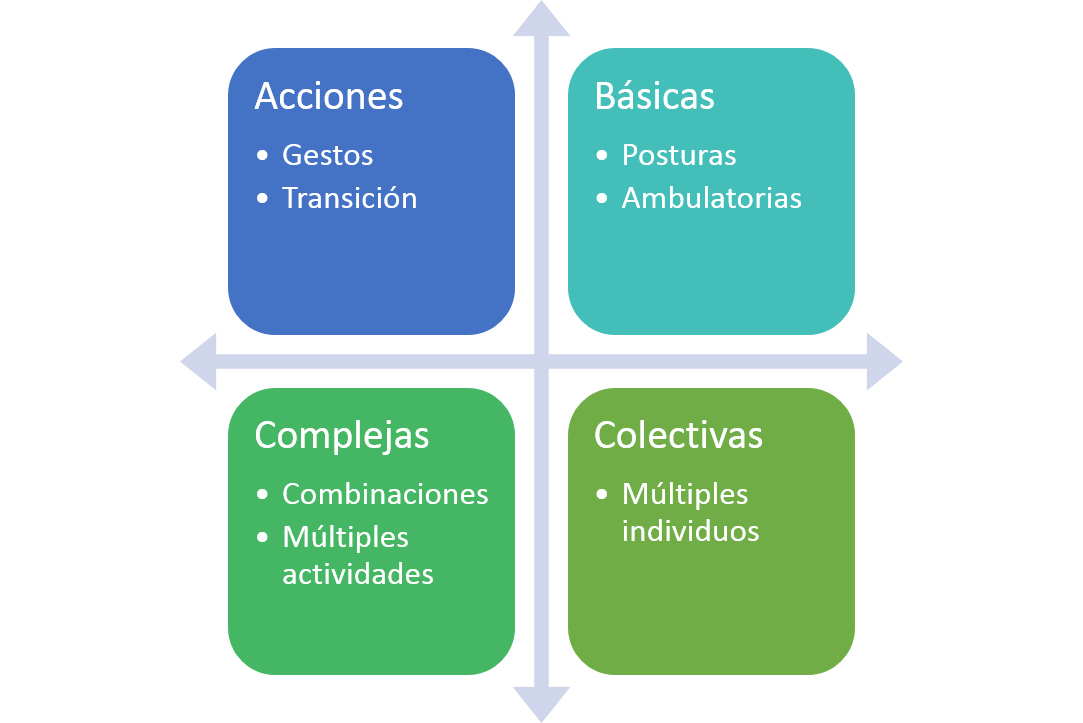
\includegraphics[width=0.95\columnwidth]{propuesta/graphics/actividades}
\par\end{center}

\begin{flushright}
{\small{}\emph{{\small{}{[}Chen et al., 2012, Reyes Ortiz, 2015{]}}}}
\par\end{flushright}{\small \par}

\end{columns}

\end{frame}
%
\begin{frame}{Actividades Humanas}

\framesubtitle{Alcance}

\resizebox{0.75\textwidth}{!}{

\noindent\begin{minipage}[t]{1\columnwidth}%
\begin{tabular}{l|>{\raggedright}p{5cm}|>{\raggedright}m{6cm}}
\textbf{Grupo}  & \textbf{Actividades}  & \textbf{�reas de Aplicaci�n}\tabularnewline
\hline 
Posturas & Sentado

Parado

Acostado & Medicina, Cuidado Personal, Asistencia en vida diaria\tabularnewline
\hline 
Ambulatorias  & Caminar

Correr

Quieto

Subir y descender escaleras & Cuidado Personal, Entretenimiento\tabularnewline
\hline 
Transporte  & \noindent En bus o autom�vil

\noindent En bicicleta & Conmutar, Seguridad\tabularnewline
\hline 
Cotidianas & \noindent Comer

\noindent Beber

\noindent Trabajar en la PC

\noindent Mirar TV

\noindent Leer un libro  & Asistencia en la vida diaria, Ambientes inteligentes\tabularnewline
\end{tabular}%
\end{minipage}

}
\end{frame}

